\documentclass[crop, tikz]{standalone}
\usepackage{tikz}

\usetikzlibrary{positioning, shapes}

\begin{document}
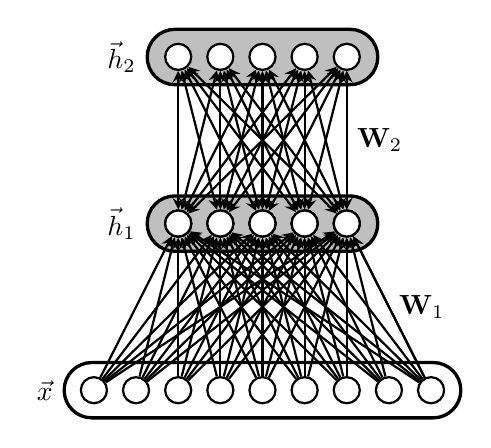
\begin{tikzpicture}

	\node (1) [draw, minimum width=15em, minimum height=2em, very thick, rounded rectangle] {};
	\node (l1) [left=0em of 1] {$\vec{x}$};
		
	\node (2) [above=3.9em of 1, draw, fill=lightgray, minimum width=9em,very thick, minimum height=2em, rounded rectangle] {};
	\node (l2) [left=0em of 2] {$\vec{h}_1$};
	\node (3) [above=3.9em of 2, draw, fill=lightgray, minimum width=9em,very thick, minimum height=2em, rounded rectangle] {};
	\node (l3) [left=0em of 3] {$\vec{h}_2$};
		
	\node[circle, draw, thick] (A1) {};
	\node[circle, draw, thick, right=0.5em of A1] (A2) {};
	\node[circle, draw, thick, right=0.5em of A2] (A3) {};
	\node[circle, draw, thick, right=0.5em of A3] (A4) {};
	\node[circle, draw, thick, right=0.5em of A4] (A5) {};
	\node[circle, draw, thick, left=0.5em of A1] (A6) {};
	\node[circle, draw, thick, left=0.5em of A6] (A7) {};
	\node[circle, draw, thick, left=0.5em of A7] (A8) {};
	\node[circle, draw, thick, left=0.5em of A8] (A9) {};
		
	\node[circle, draw, fill=white, thick, above=5em of A1] (B1) {};
	\node[circle, draw, fill=white, thick, right=0.5em of B1] (B2) {};
	\node[circle, draw, fill=white, thick, right=0.5em of B2] (B3) {};
	\node[circle, draw, fill=white, thick, left=0.5em of B1] (B4) {};
	\node[circle, draw, fill=white, thick, left=0.5em of B4] (B5) {};
		
	\node[circle, draw, fill=white, thick, above=5em of A1] (B1) {};
	\node[circle, draw, fill=white, thick, right=0.5em of B1] (B2) {};
	\node[circle, draw, fill=white, thick, right=0.5em of B2] (B3) {};
	\node[circle, draw, fill=white, thick, left=0.5em of B1] (B4) {};
	\node[circle, draw, fill=white, thick, left=0.5em of B4] (B5) {};
		
	\node[circle, draw, fill=white, thick, above=5em of A1] (B1) {};
	\node[circle, draw, fill=white, thick, right=0.5em of B1] (B2) {};
	\node[circle, draw, fill=white, thick, right=0.5em of B2] (B3) {};
	\node[circle, draw, fill=white, thick, left=0.5em of B1] (B4) {};
	\node[circle, draw, fill=white, thick, left=0.5em of B4] (B5) {};
		
	\node[circle, draw, fill=white, thick, above=5em of B1] (C1) {};
	\node[circle, draw, fill=white, thick, right=0.5em of C1] (C2) {};
	\node[circle, draw, fill=white, thick, right=0.5em of C2] (C3) {};
	\node[circle, draw, fill=white, thick, left=0.5em of C1] (C4) {};
	\node[circle, draw, fill=white, thick, left=0.5em of C4] (C5) {};
		
	\foreach \x in {1,...,9}
		\foreach \y in {1,...,5}
			\draw[-stealth, thick] (A\x) -- (B\y);
				
	\foreach \x in {1,...,5}
		\foreach \y in {1,...,5}
			\draw[stealth-stealth, thick] (B\x) -- (C\y);
				
	\draw[-stealth, thick] (A5) -- node[right] {${\bf W}_1$} (B3);
	\draw[stealth-stealth, thick] (B3) -- node[right] {${\bf W}_2$} (C3);
	
\end{tikzpicture}
\end{document}